\documentclass[twocolumn]{aastex63}
\usepackage{float}
\newcommand{\vdag}{(v)^\dagger}
\newcommand\aastex{AAS\TeX}
\newcommand\latex{La\TeX}

\begin{document}

\title{Tidal Evolution of M33's Dark Matter Halo—Mass loss of Dark Matter and changes to internal dark matter profile}

\author{Yuxuan Chen}
\affil{Steward Observatory, University of Arizona, 933 North Cherry Avenue, Tucson, AZ 85721, USA}
\date{May 2020}
\begin{abstract}
 This project is to investigate the tidal evolution of M33's dark matter halo through the mass loss of M33 dark Matter and change to M33 internal dark matter profile. mass loss of the dark matter halo will help us to understand the evolution of satellite galaxies (like M33) which are affected by strong tides.The change of the dark matter mass of the galaxy controls the evolution of the galaxy, because the morphology and kinematics structures of galaxies consequently change due to lose dark matter. The specific tasks of this project are to prove that M33 will lose dark matter mass in M33 dark matter halo, and change internal dark matter profile.If these two task are proved, they will predict the evolution of M33's dark matter halo in the future. In this project, the simulations of Jacobi Radius and Hernquist profile demonstrate the dark matter mass loss rate of M33 and the evolution of M33 internal dark matter mass profiles. The results of the simulations represent that M33 can not keep more its baryons and shrink in size. 
\keywords{Dark Matter Halo,Satellite Galaxy,Local Group, Jacobi Radius, Tidal Stripping, Spiral Galaxy, Hernquist Profile}
\end{abstract}
\section{Introduction}
The spiral galaxy M33, which is located in the constellation Triangulum, is the third largest member of our Local Group of galaxies. Also, M33 and M31 are the closest massive galaxies to the Milky Way, and all of these galaxies(MW,M31,M33) are spiral galaxy. There is large amounts of dark matter which is expected to dominate these galaxies, particularly in the outskirts of galaxies' disks, according to optical measurement of the rotation of spiral galaxies \citep{blok10}. As indicated by the project entitled "orbital analysis an velocity measurements" which is presented in van der Marel 2012, M31 and the MW will merge at t = 5.86 Gyr \citep{marel12}. In the process of merging, the orbit of M31&MW and the orbit of M31&M33 will reduce with time, so these galaxies become closer to each other.Thus, the shorter orbits of M31&MW and M31&M33 will result in stronger gravitational interactions between the MW, M31 and M33. In other words, stronger gravitational interactions between galaxies will render the impact of tidal fields between galaxies stronger, which will consequently change the morphology and kinematics of the inner and outer structures of all galaxies. In addition, the bound mass of a smaller satellite galaxy (like M33) will decrease over time, due to the tidal field of a massive galaxy\citep{boylan11}. Given that, this project is to investigate the tidal evolution of M33's dark matter halo, emphasizing on two points: 1.mass loss of dark matter, 2.change of internal dark matter profile. \\ 
\indent Dark matter has long been a much-contested topic in the area of astronomical sciences. The majority of mass in the universe is in the form of dark matter. According to the cold dark matter theory, dark matter can only interact with baryons via gravity. As dark matter predominates the mass of galaxies, dark matter will control the gravitational filed of galaxies or the depth of potential well. If the total mass of dark matter decreases in the galaxy, the galaxy will not retain part of its baryons nor accrete more gas. In other words, the change of the total dark matter mass of the galaxy controls the evolution of the galaxy. Therefore, studying the mass loss of the dark matter halo will help us to understand the evolution of satellite galaxies (like M33) which are affected by strong tides. \\
\indent After t = 10 Gyr, the MW and M31 will formed a merged remnant, and M33 will lose 23.5percent of its stars which, in other words, will be stripped off from M33 (see the first graph on the right of figure1) \citep{marel12}.  This result indicates that the mass of M33 will lose due to the tidal evolution of MW and M31 merger process. Elsewhere, in Boylan Kolchin et al(2012)'s research, astronomers could potentially detect the signal of dark matter annihilation, if the internal dark matter density becomes high enough\citep{boylan11}. If the internal dark matter density of a satellite decreases, the expected annihilation signal will be lower. So the change of internal dark matter density profile of a satellite galaxy(like M33) is very important to indicate whether astronomers can detect the signal of dark matter annihilation so as do the future dark matter detection experiments.  Then, the questions will be focusing on M33.\\

\indent Boylan Kolchin et al.(2012) is indeed inspirational for this project. Is the central dark matter density profile of M33 sufficiently high enough to produce a dark matter annihilation signal? And will that density profile change in the future? Everything related to dark matter is still an intriguing question. However in this project, the mainly focus is to study that how does the tidal evolution of M33&M31&MW system impact the M33 dark matter halo through the mass loss of M33 dark Matter and change to M33 internal dark matter profile based on the limited evidence I have. 
\begin{figure}[H]
    \centering
    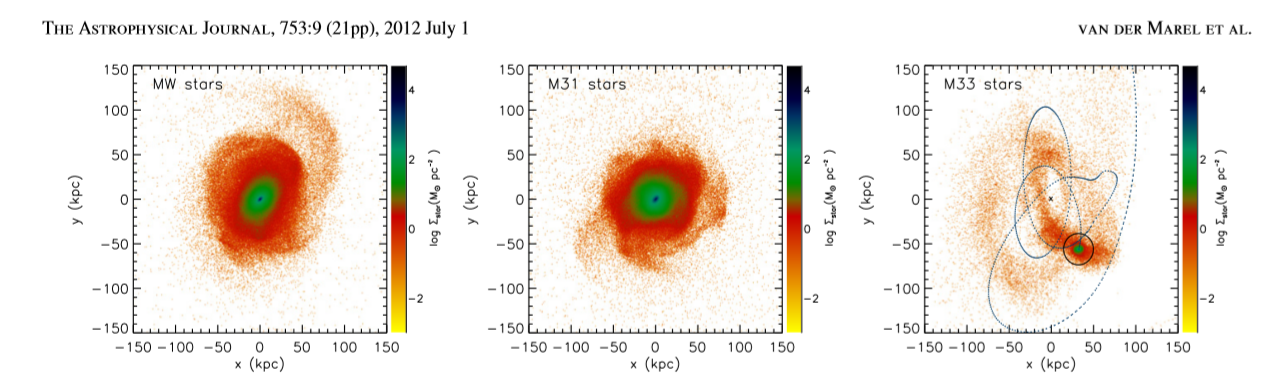
\includegraphics[width=7cm]{f1.png}
    \caption{The graph illustrates the mass distribution of the MW, M31 and M33 in the final snapshot of the simulation, when the MW and M31 coalesced. The final snapshot of the M33 simulation is on the very right. In the last simulation Snapshot of M33, 23.5 percent stars of M33 that will be stripped from M33. Much mass per particle is outside the Jacobi radius of M33 \cite{marel12}.}
    \label{marelfigure}
\end{figure} 
\section{This Project} 
\indent In this paper will study the change of M33's dark matter halo profile and internal dark matter profile during the period of M31 and M33's orbit evolution. I will simulate the outer/internal dark matter mass profile and internal density disk/dark matter halo profile of M33 based on the simulation data of the merger of M31 and MW.
\indent The specific task of this project is to prove that M33 will lose dark matter mass due to the tidal influence from M31 and M33, and to show the change of mass loss rate of M33 as function of time. Next, to prove whether the mass profiles of M33 will decay in the future is also a question that this project need to solve. The other goal is to understand what happened to internal dark matter density profile of M33, and whether it will change. In addition, the dark matter density profile of M33 which I calculated is mean density profile; it is necessary to check the result through Hernquist mean density profile.   \\
\indent As detailed in the introduction, the dark matter will control the gravitational field or the depth of potential well of galaxies. Therefore, the change of M33 dark matter total mass matters whether M33 will lose its baryons or accrete less gas in the future. Also, it is important to know the change of M33 dark matter halo mass profile to predict the evolution of M33. In addition, if the internal dark matter density profile of M33 is high enough to produce a dark matter annihilation signal, then astronomers can do dark matter detection experiments of M33 in future. 
\section{Methodology} 
\indent This project will simulate Jacobi Radius of M33 based on the tidal effect acting on M33 which is from M31 or the merger of MW&M31. The Jacobi Radius simulation means the maximum radius that a satellite galaxy(like M33) can extend due to the expected tidal radius. In order to do the simulation of Jacobi Radius, the mass of satellite galaxy(like M33) and host galaxy has to be calculated. Therefore, I will make a program to compute Jacobi Radius as function of time. Meanwhile, this project will also use the simulation of enclosed mass profile to simulate the M33 dark matter mass profile. The simulation displays the distribution of galaxy (like M33) mass as function of radius(in kpc), so it is necessary to make a program to plot M33 mass profiles of different periods in order to check the mass loss of M33. In addition, according to the M33 dark matter mass profile, the M33 dark matter mean density profile can be calculated. Thus, the project will use the simulation of Hernquist mean density profile based on Hernquist Profile.The Hernquist Profile considered that the dynamical and tidal effects are from the mergers of galaxies which are acting on the satellite galaxies, so it is more accurate to check whether the M33 mean density profile is correct through Hernquist profile. 
\begin{figure}[H]
    \centering
    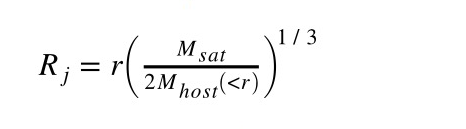
\includegraphics[width=3.5cm]{JacobiRadius.png}
    \caption{Jacobi radius based on tidal radius of host mass}
\end{figure}
\indent In order to simulate M33 Jacobi Radius, the host galaxy mass and satellite galaxy mass have to be specifically defined (as shown on Figure 2). It is widely believed that only mass of M31 has to count into the host mass before the merger of M31 and MW, because M31 is the only massive galaxy closest to M33 which results in gravitational interaction. As mentioned in van der Marel 2012 that M31 and the MW will merge after t = 5.86 Gyr \citep{marel12}, so both the mass of MW and M31 will be counted into the host mass in order to calculate M33 Jacobi Radius after the merger of MW and M31(I select t = 6,5 Gyr). Then, to make a plot of "Jacobi Radius vs Time" is to check whether the Jacobi Radius decreases, according to the 800 snapshots files of M33,M31 and MW orbit simulation which Prof. Gurtina,Besla provided.If the Jacobi radius is decreasing as function of time, examining how much mass is inside the Jacobi radius as function of time can demonstrate the mass loss rate and cumulative mass loss fraction as function of average time more obviously. In addition, in 800 snapshot files, the mass of M33 was recorded as mass per particle for each recorded coordination, which is simulated from the position of M33 orbit. Thus, I can create the dark matter halo mass profiles based on different files. After that, the internal(the range is the Jacobi Radius of Snapshot 800) dark matter mean density profile of M33 can be plotted. In order to make Hernquist mean density profile to check the result, I will use a program to find the best scale radius for the Hernquist profile. \\
\begin{figure}[H]
    \centering
    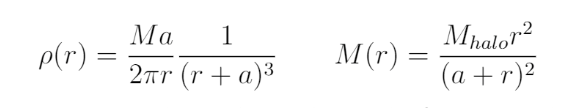
\includegraphics[width=4.5cm]{Hernquist Equation.png}
    \caption{Hernquist Mass Profile\cite{Hernquist}.}
    \label{Hernquistfigure}
\end{figure}

\indent First of all, according to Jacobi Radius equation, I have to define two equations in the code. The first one is to count mass per particle, which is in the range between center of mass position of M33 and M31, as host mass from M33 reading files (adding MW mass and reading MW files after t = 6.5 Gyr). The second one is to count mass per particle, which is in Jacobi radius of M33, as satellite mass. Next, I have to initialize the Jacobi radius, because I do not know M33's Jacobi radius. I will regard the first satellite mass as the initial Jacobi mass, and use the first host mass to get initial Jacobi radius. After that, I will bring the initial Jacobi radius as the index to Jacobi mass equation, when it is reading the second snapshot. And I can see how much mass per particle is still in the initial Jacobi radius, and get new Jacobi mass. Through new Jacobi mass and second host mass, I will get new Jacobi radius. Thus, I can bring it to the third snapshot and repeat above steps, but I need to write a "if condition" for adding the mass of MW when "t = 6,5 Gyr". Until the end of the "for loop", the program will text Jacobi Mass(1e10M\textsubscript{\(\odot\)},Time(Gyr), and Jacobi Radius(kpc) out to new data file.Then, those data can be used in plotting. Additionally, writing a new program is to read the mass data from the snapshot files which I will select the files when the Jacobi Radius is in local minima. After reading those data, the mass profiles of M33 in different local minima of Jacobi radius can be plotted. In addition, through dividing the spherical volume, the M33 mean density mass profile can be plotted from the M33 mass profiles. In the end, I will plot the Hernquist mean density profiles with each mean density profiles separately after calculating the best fitted scale radius of each M33 mean density profiles.\\
\indent After plotting the Jacobi Radius vs time plot, if the mass of M33 loses, the Jacobi Radius will decrease. In order to get detail of mass loss, examining how much mass is inside the Jacobi radius as function of time from "Jacobi Radius vs Time", can demonstrate the mass loss or mass loss rate as function of average time more specifically. The M33 dark matter halo mass profiles plots(when Jacobi Radius are at local minima), where M33 is near its Perihelion of M33 and M31 orbit , can directly prove whether the mass of M33 dark matter halo lose through checking the mass distribution of these plots on the same radius(kpc). In addition, it can infer whether the dark matter annihilation will be observed in the future through checking the change of these mean density profile plots. \\

\indent The first hypothesis of this project supports that total mass of M33 will become smaller, and the amount of M33 dark matter will decrease as function of time. The second hypothesis of this project is that the decay of the dark matter distribution of M33 is tenable, because the gravitational balance of M33 itself has broken due to the stronger tidal effect of M31 or the merger of M31 and MW. Thus, part of M33 dark matter mass will strip out of M33. And the internal dark matter mass profile will decrease, because the Jacobi Radius decreased that shorted the internal range of M33.  

\section{Result} 
\indent This figure(figure4) is 'Jacobi Radius vs time', I have also plotted the M31 and M33 orbit on the plot. In order to see what happened in each step, I made the radius of M31 and M33 ten times smaller. As indicated in Figure 4, Jacobi radius is larger at aphelion of the orbit of M31 and M33,  and smaller at perihelion of the orbit of M31 and M33. And the totally trend of "Jacobi Radius vs time" tends to decrease as function of time. 
\begin{figure}[H]
    \centering
    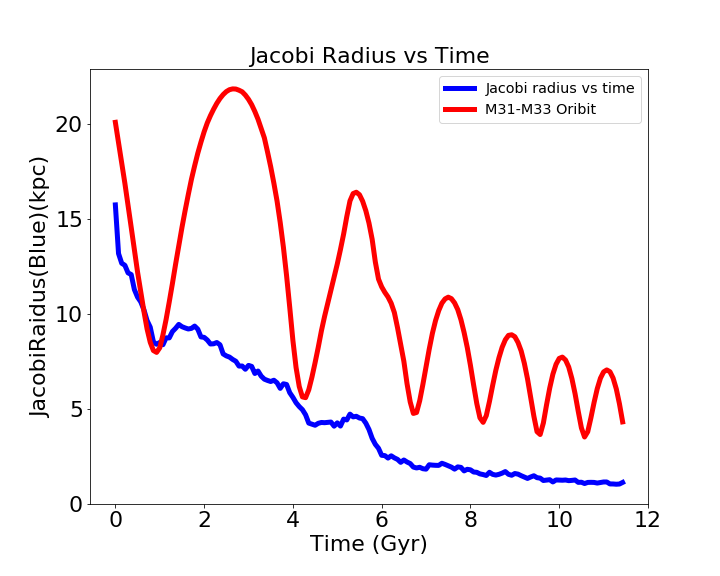
\includegraphics[width=3.5cm]{JacobiRadiusVSTime.png}
    \caption{Jacobi radius vs Time, y axis is distance in kpc, x axis is time in Gyr. The blue line is Jacobi radius vs time, the red line is the diameter of M31 and M33 orbit vs time. the result I put ten times smaller M31 and M33 orbit is to show the relation between each time step more obviously.}
\end{figure}

As indicated in Figure 5(M33 Average time vs Mass loss Rate), when the mass loss rate is below zero, M33 will lose part of its mass. And when the mass loss rate is greater than zero, M33 will add mass to itself. The overall trend of mass loss rate as function of average time tends to be negative which M33 will lose mass as function of time. However, there are several values of mass loss rate which are positive   \\

\begin{figure}[H]
    \centering
    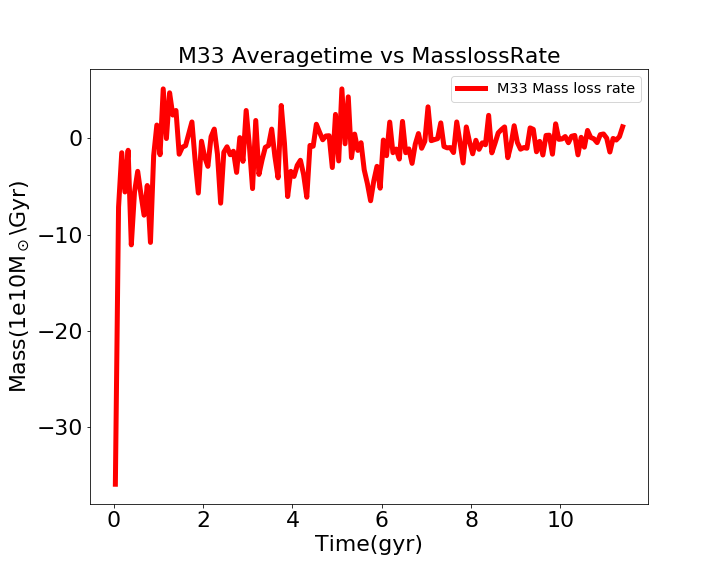
\includegraphics[width=4cm]{M33MassLossRate.png}\hfill
    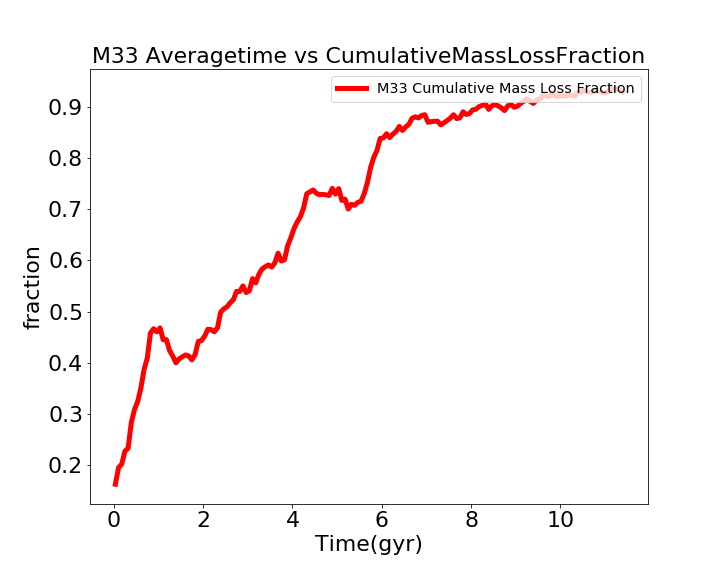
\includegraphics[width=4cm]{CumulativeMasslossfractionvsTime.png}\hfill
    \caption{The left graph shows the relation between average time and Mass loss rate, y axis is mass loss rate in unit of 1e10M\textsubscript{\(\odot\)} per Gyr, x axis is time in Gyr. The right graph is 'M33 Cumulative Mass Loss Fraction vs Time'. The unit of y axis is dimensional less, because it is fraction between the change of Jacobi Mass and initial Jacobi Mass. The x axis is time in Gyr. }
\end{figure}
The graph, "M33 Cumulative Mass Loss Fraction vs Time", directly demonstrated that the cumulative mass loss fraction of M33 will increase sharply around 0 to 6 Gyrs. And the cumulative mass loss fraction of M33 will stay around the peak ,which is 0.9, after the merger of M31 and MW(t = 6.5 Gyr).  So as time goes by, M33 will lose its mass. The mass of M33 will lose for absolutely;thus it is necessary to check the M33 mass profiles to see more details of M33 dark matter halo. \\

\indent In Figure 6, the plots of M33 mass profiles,which I took from 1 initial snapshot file and 3 snapshot files which Jacobi Radius is at local minima,are M33 dark matter halo mass profile and M33 internal dark matter mass profile.The left plot, M33 dark matter halo mass profiles, shows that the trend of M33 dark matter mass profile is tending to decrease slightly as function of time. So, the M33 dark matter halo will lose its dark matter, and M33 dark matter mass profile will change.In addition, the range of M33 internal dark matter mass profiles is around 15 kpc based on the Jacobi Radius of the last snapshot file.The plot of M33 internal dark matter mass profiles, also keeps the similarly trend as the plot of M33 dark matter halo mass profiles. Hernquist mean density profiles will show more.
\begin{figure}[H]
    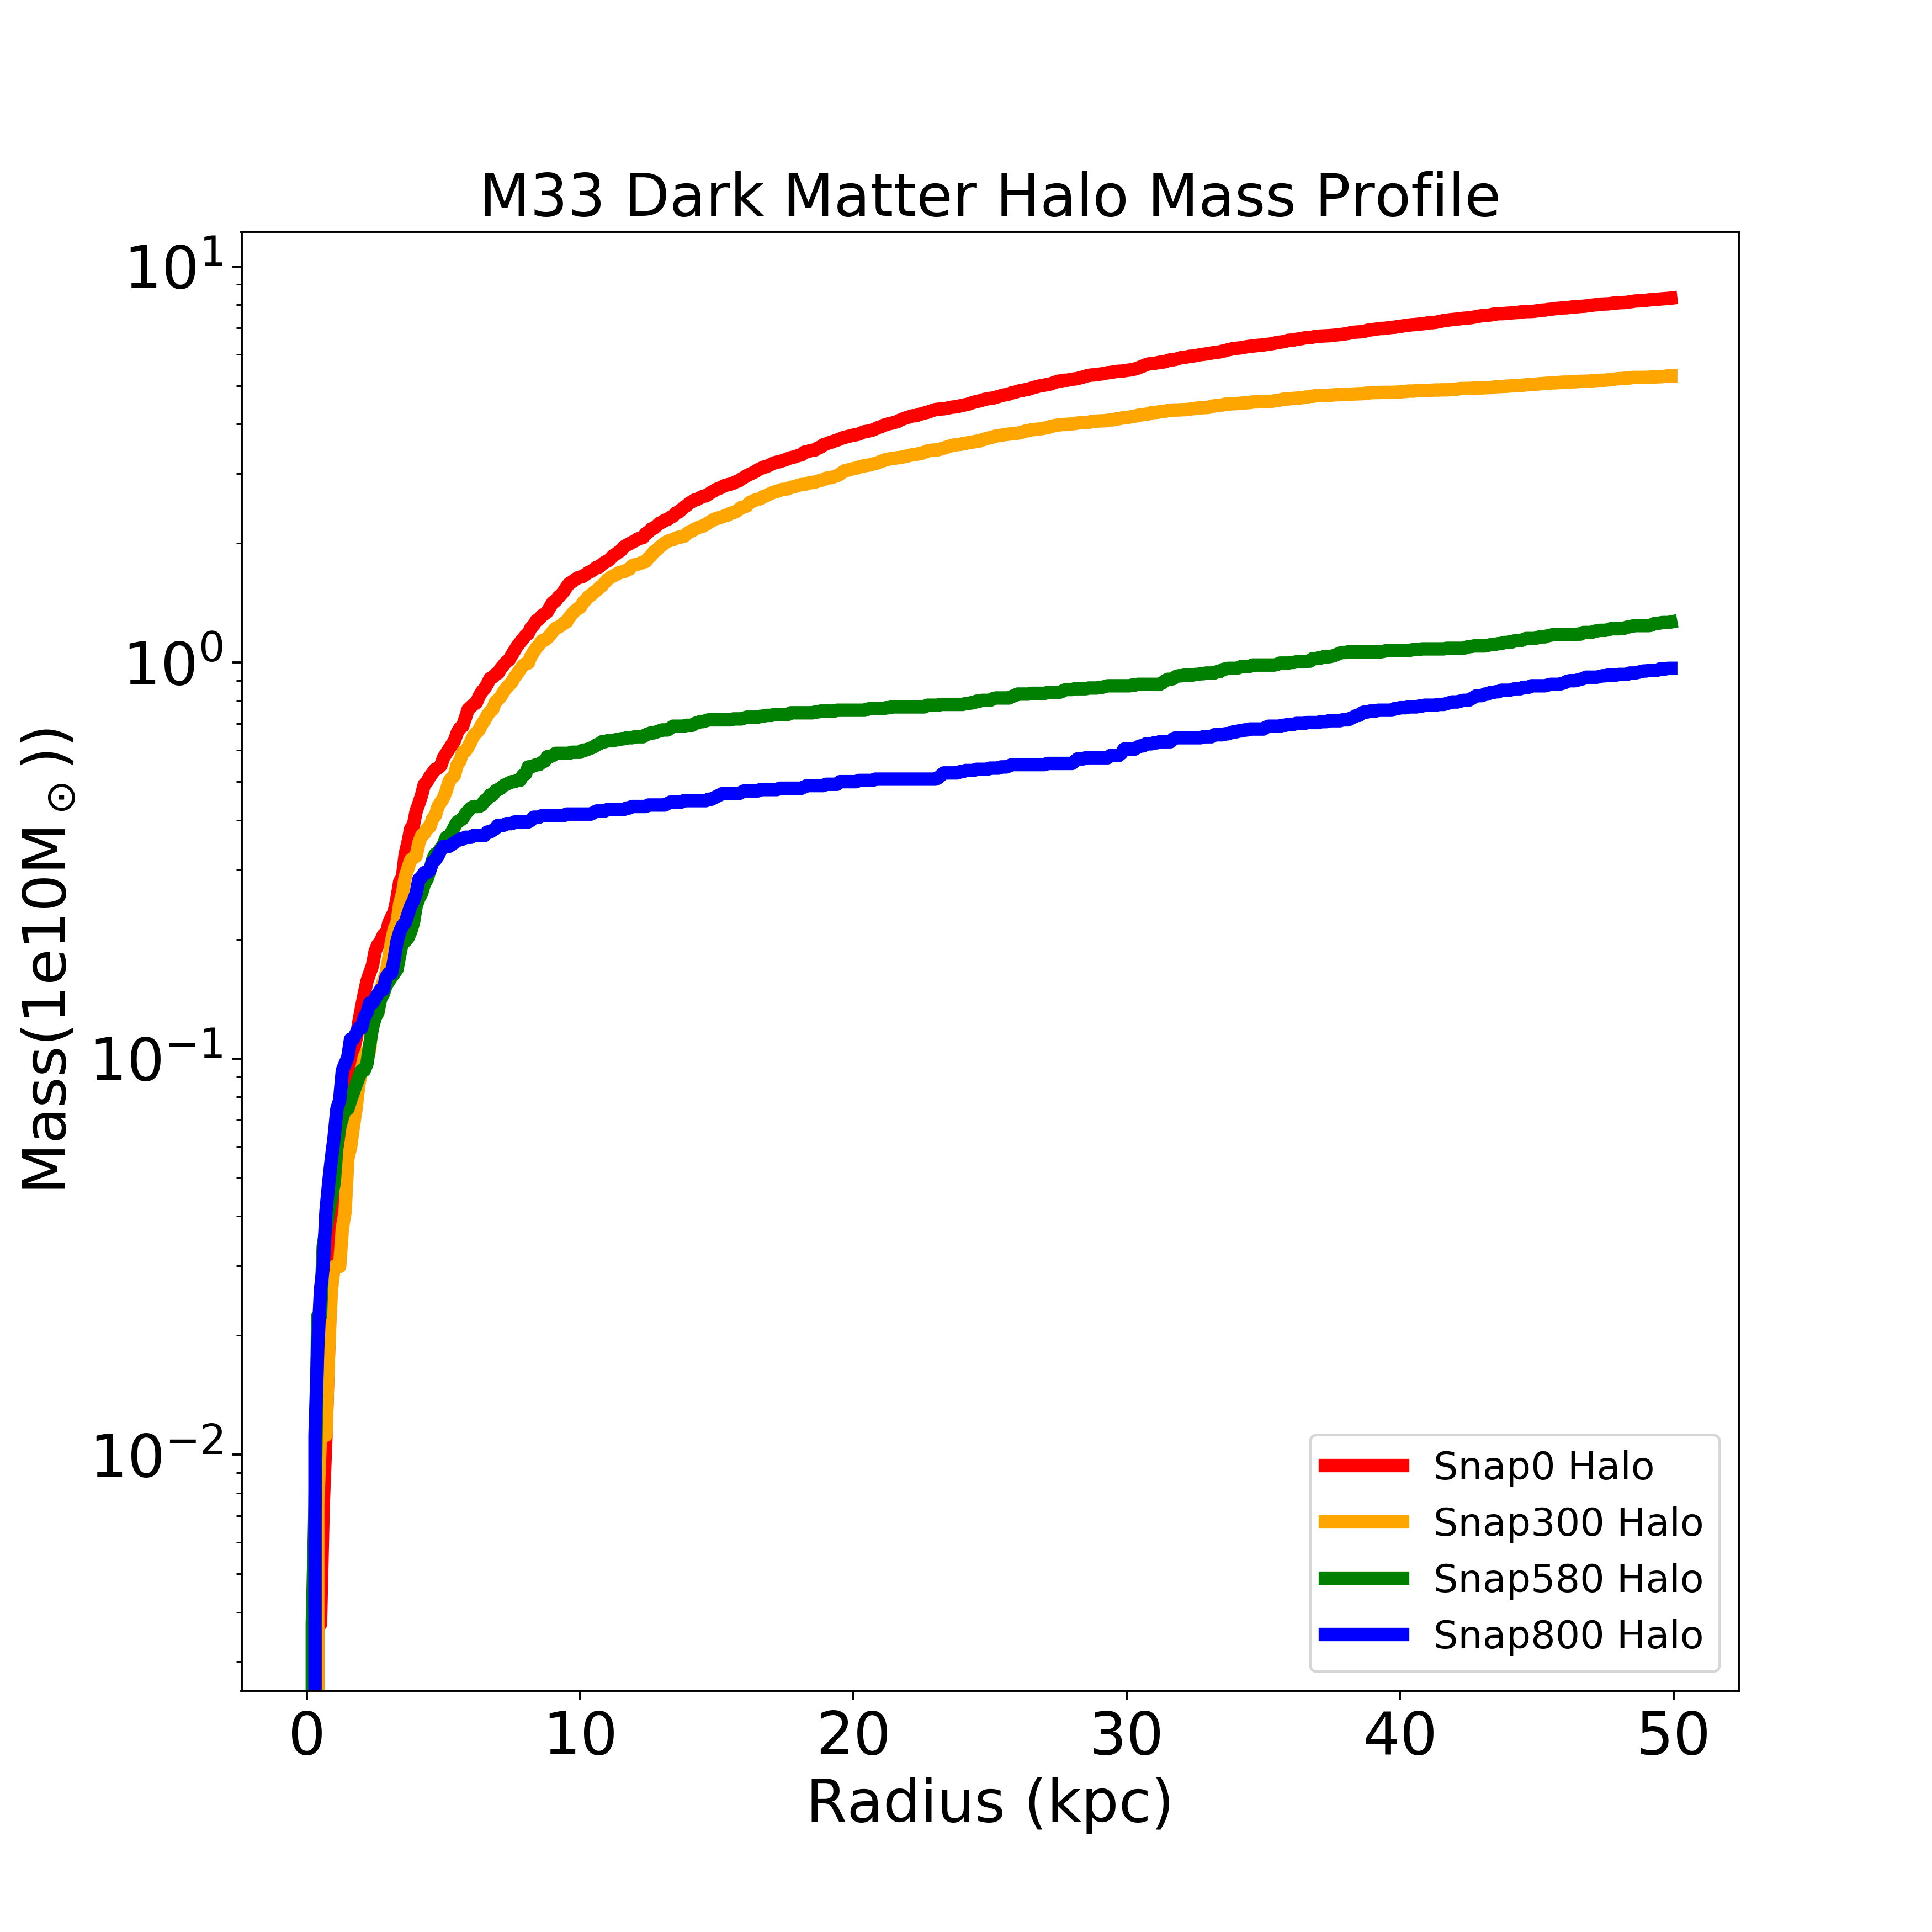
\includegraphics[width=3.5cm]{MassProfile_M33Halo.png}\hfill
    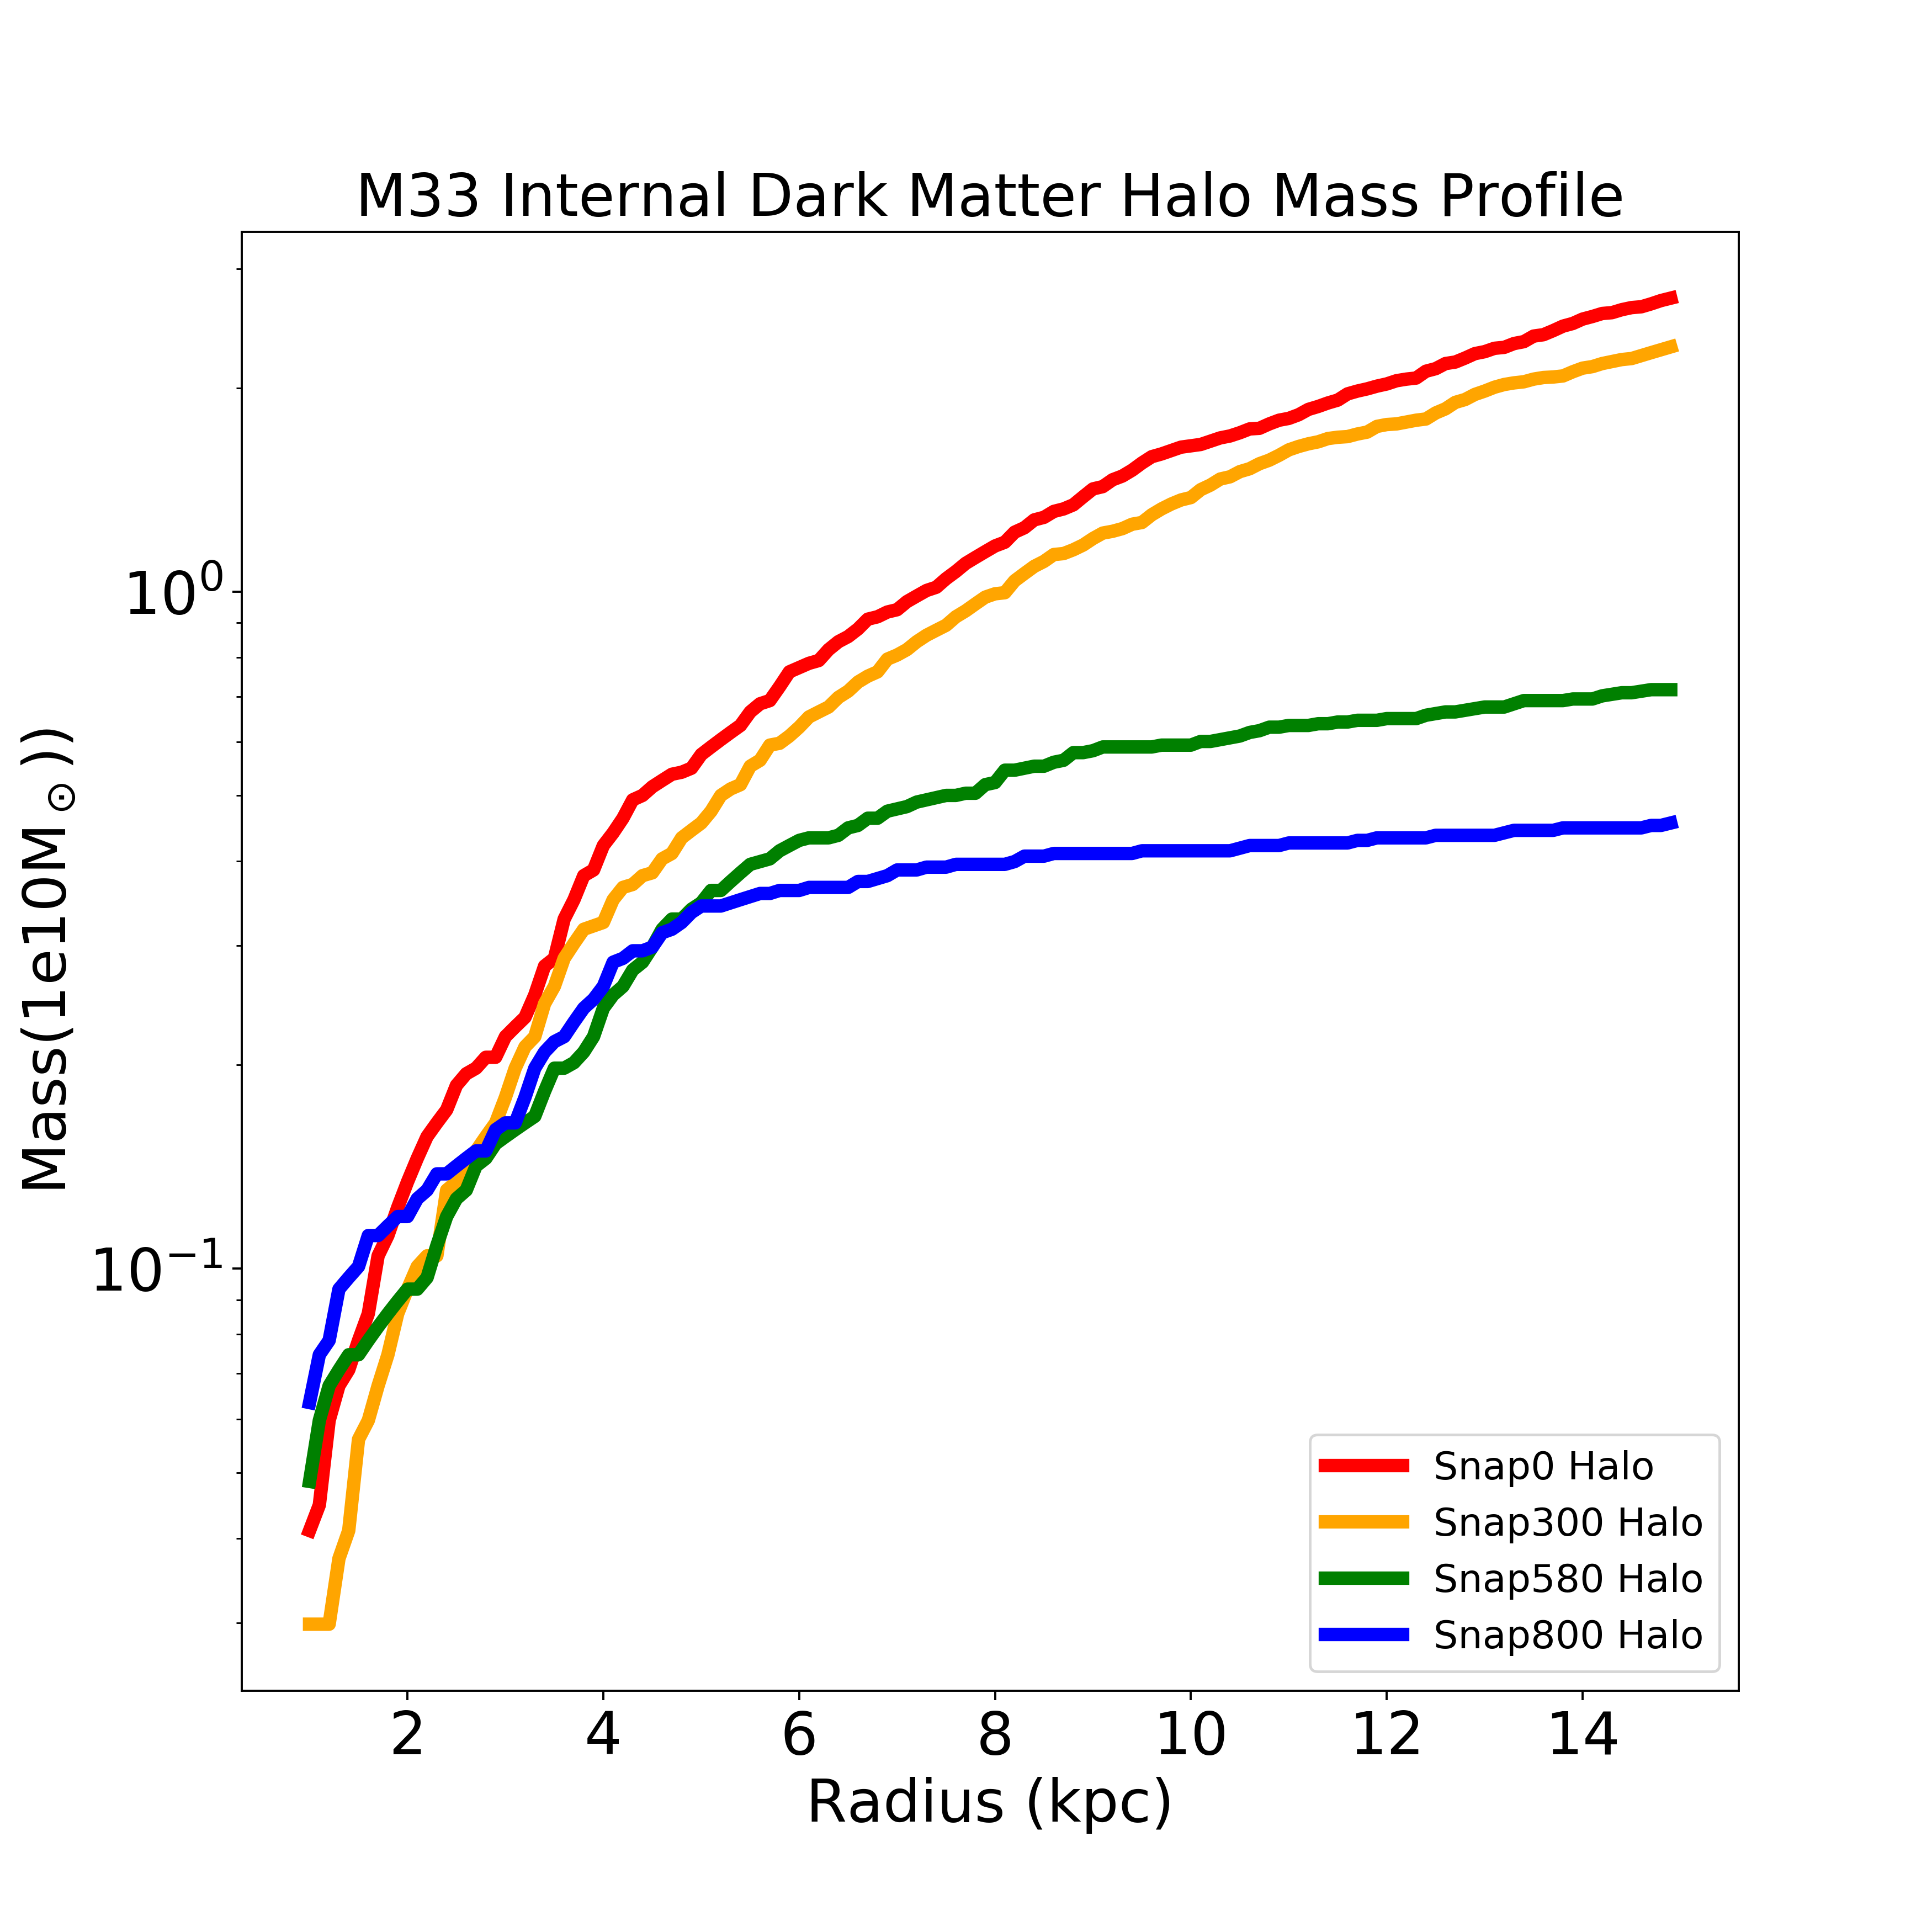
\includegraphics[width=3.5cm]{MassProfile_InternalM33Halo.png}\hfill
    \caption{The graph is M33 dark matter halo mass profile. The unit of y axis is 1e10M\textsubscript{\(\odot\)}, and x axis is radius in kpc. 1.red represents  snapshot file 0, 2. orange represents snapshot file 300, 3. green line represents snapshot file 580, and 4. blue represents snapshot file 800.}
\end{figure}
The comparison of Hernquist and M33 enclosed internal dark matter mean density is shown on Figure 7. As indicated by the Hernquist mean density profiles on Figure 8, the distributions of M33 internal dark matter mean density profiles are tending to decrease from snapshot 0 to 800(0 to 10 Gyrs). And according to the relation between mass and mean density, the M33 internal dark matter mass profiles also will decrease when radius is smaller than 4 kpc, so the actual Jacobi Radius is larger than the value of Jacobi Radius simulation. Moreover, the chance of the observation of dark matter annihilation in M33 center will decrease. 
\begin{figure}
    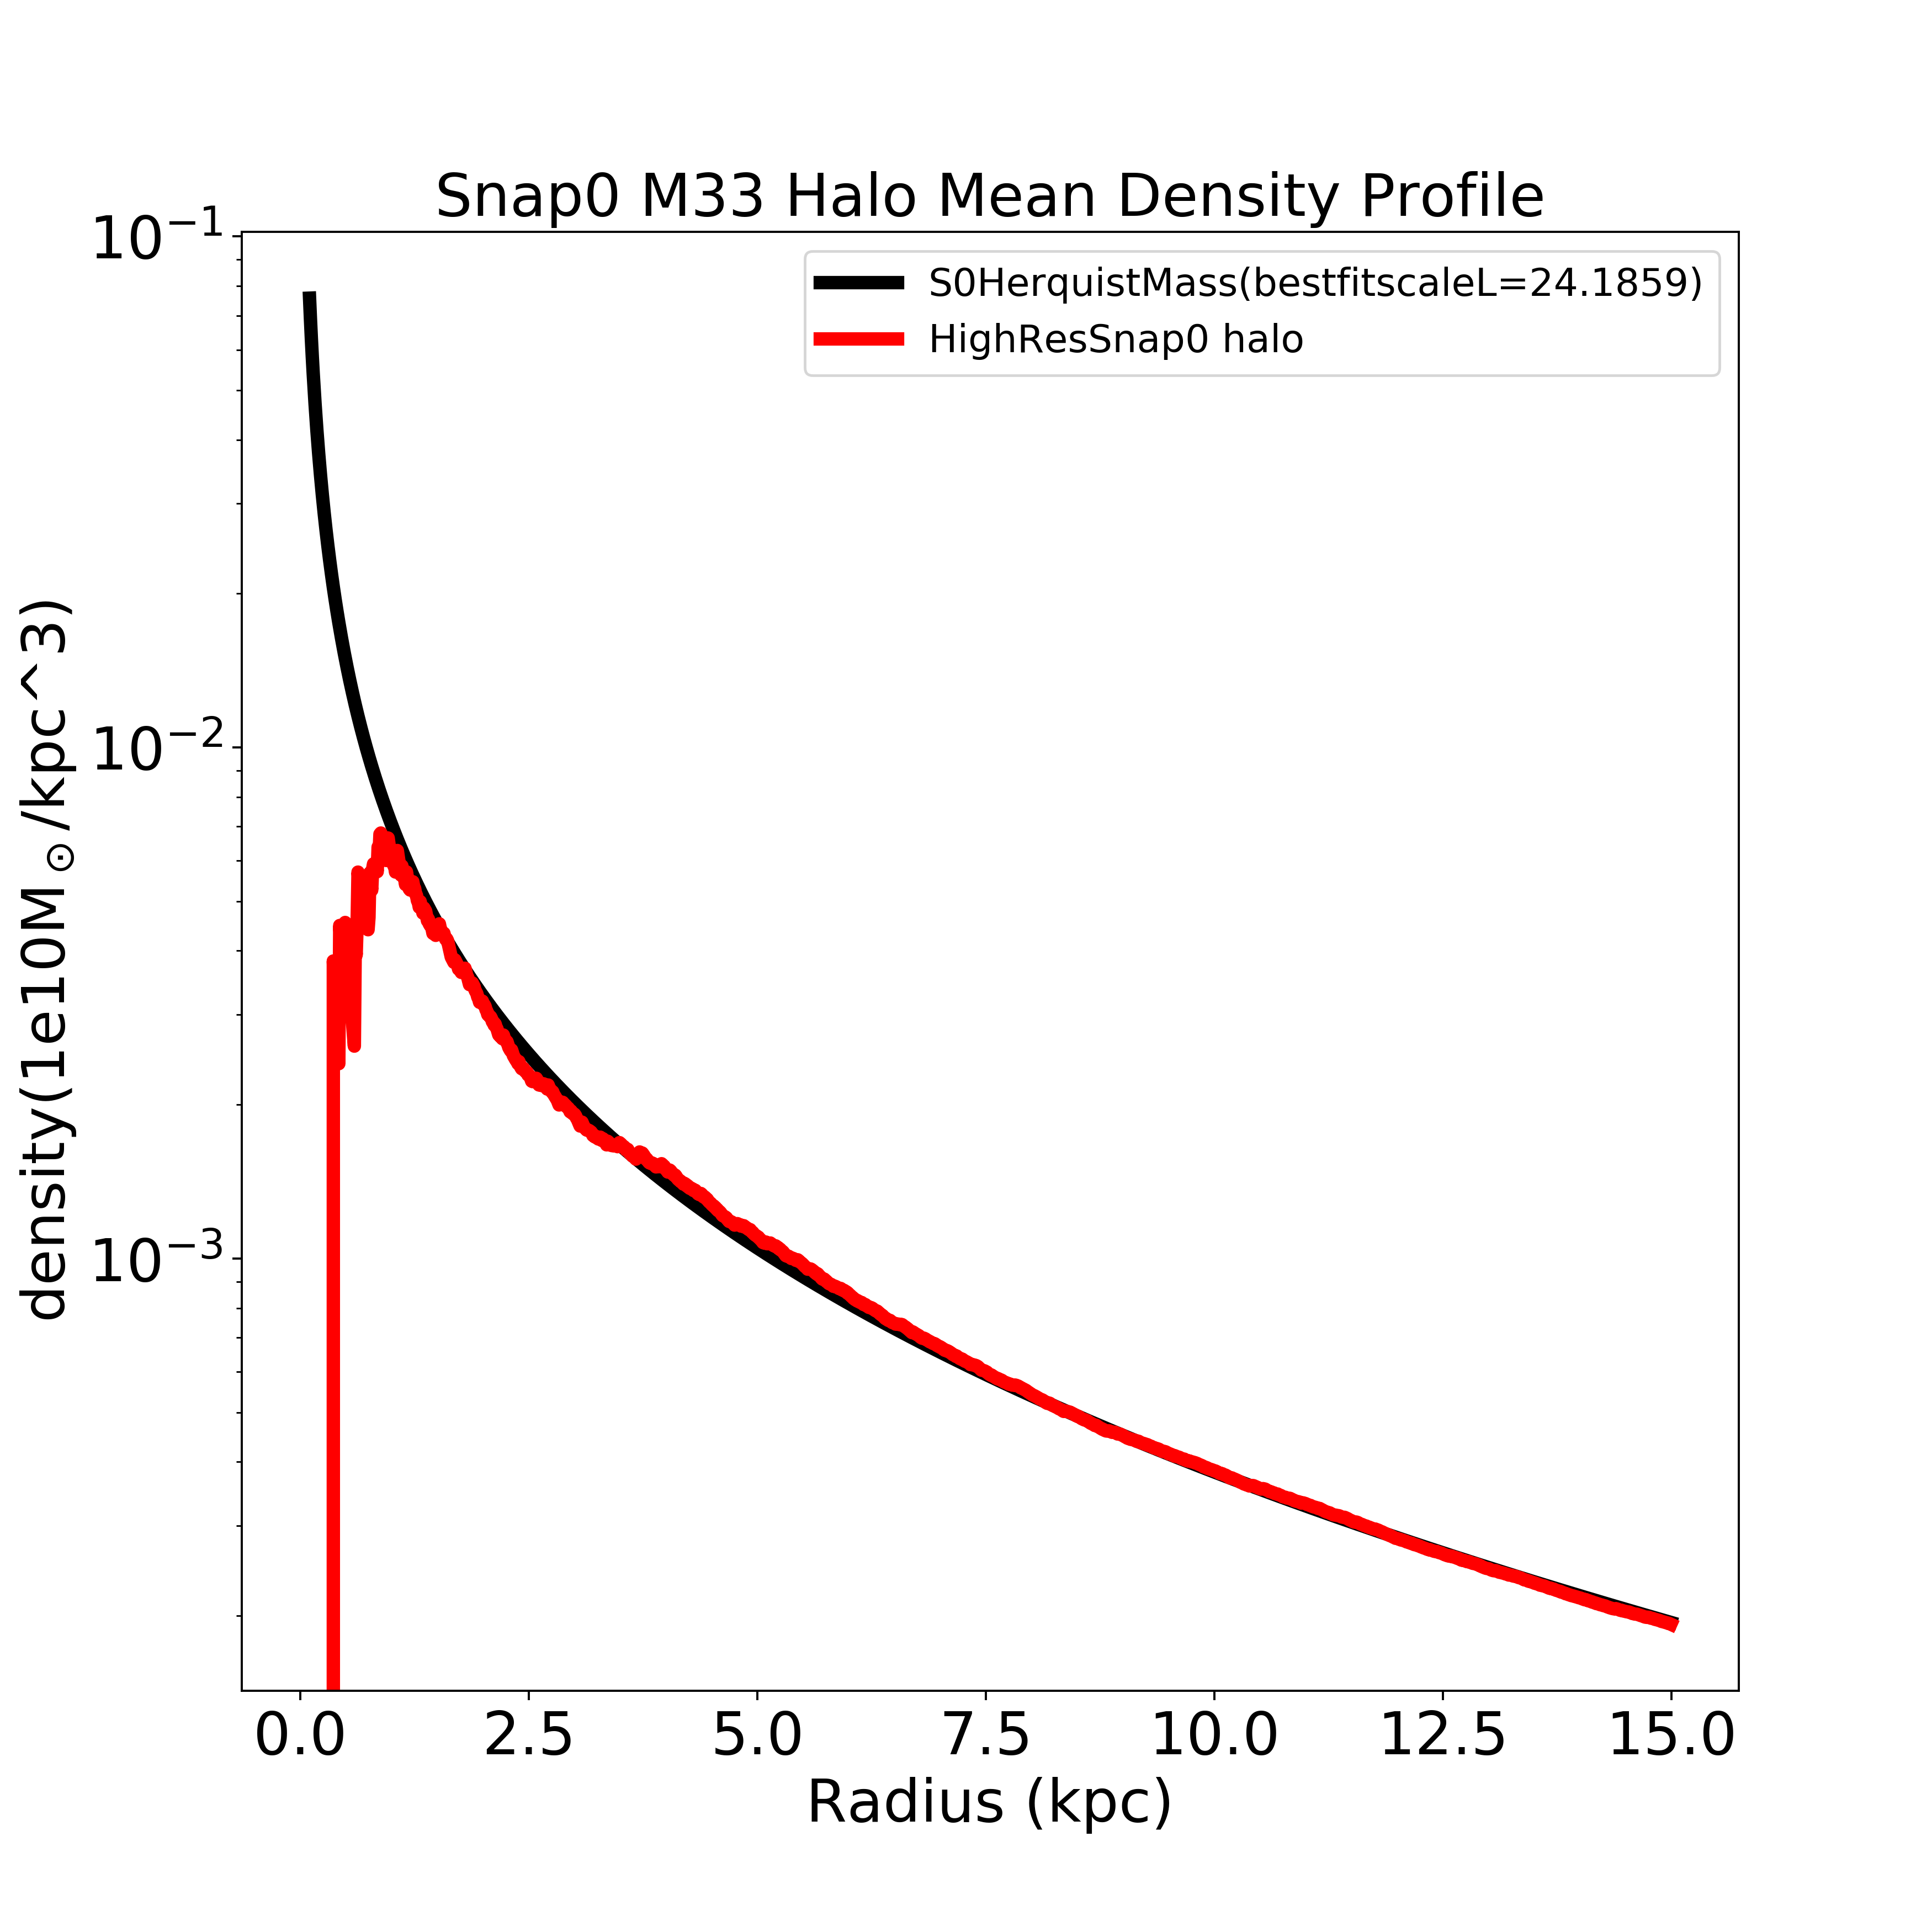
\includegraphics[width=2cm]{Snapshot0EnclosedvsHernquistMeanDensity.png}\hfill
    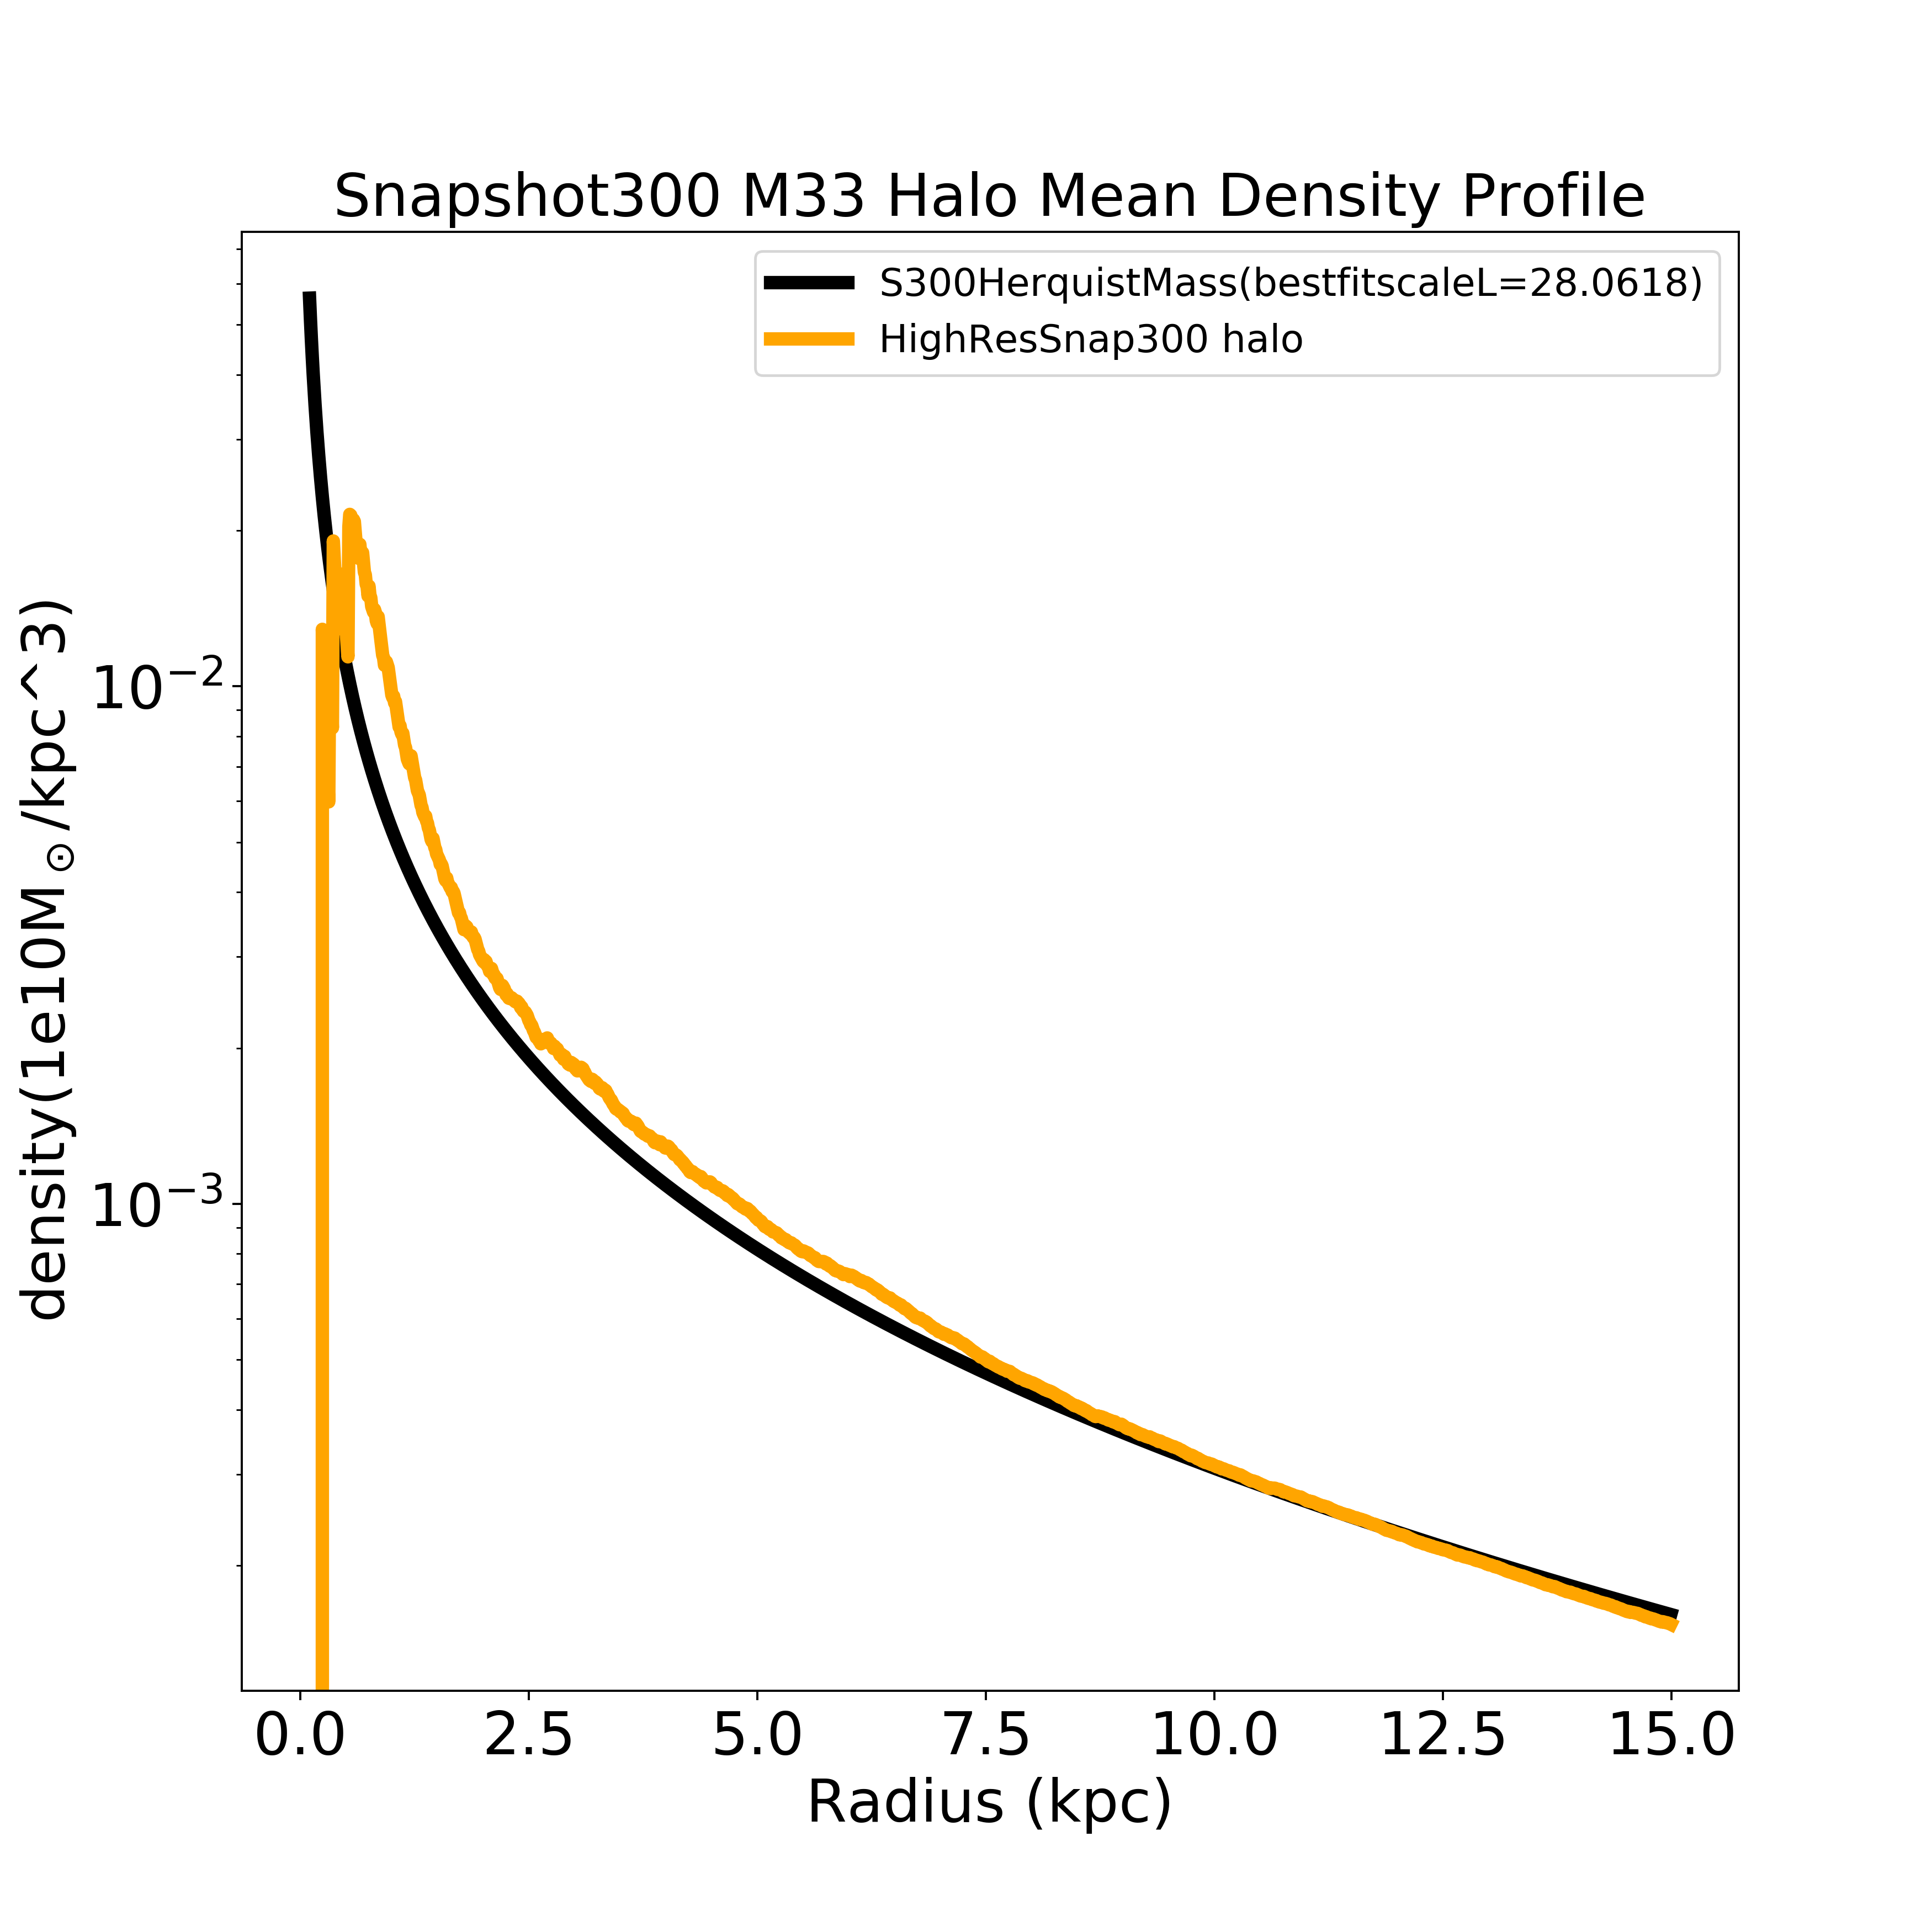
\includegraphics[width=2cm]{Snapshot300EnclosedvsHernquistMeanDensity.png}\hfill
    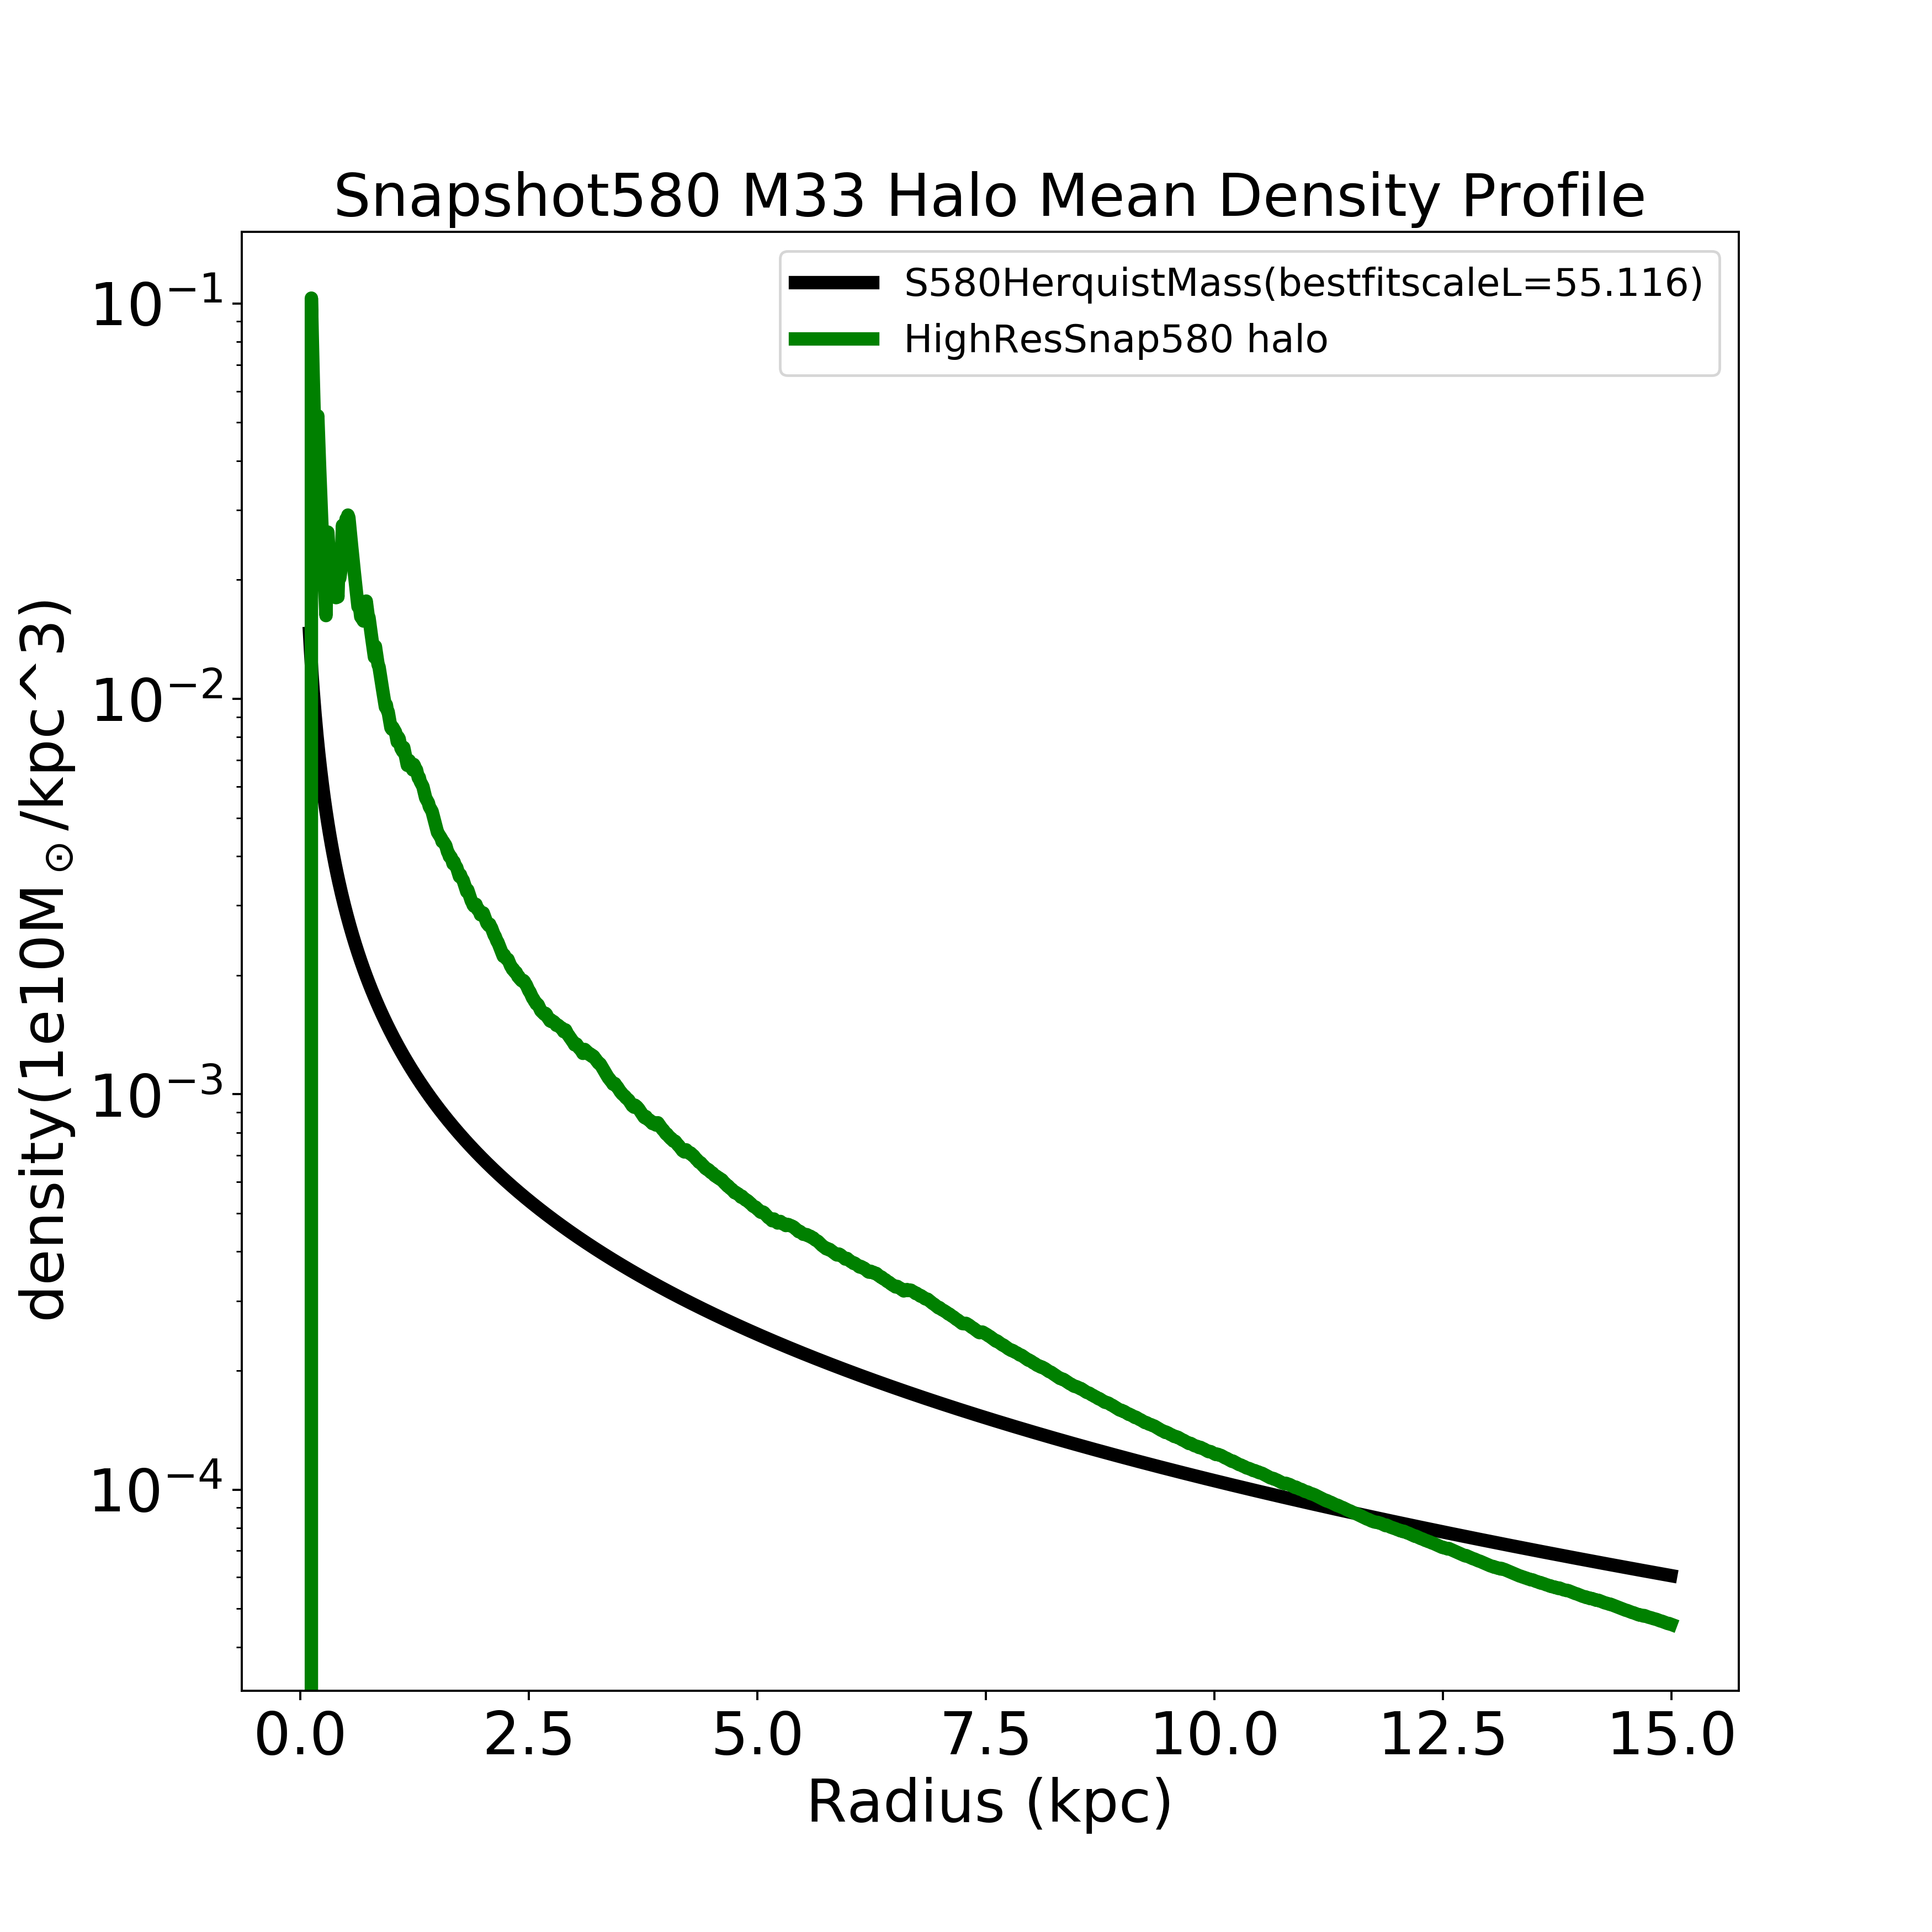
\includegraphics[width=2cm]{Snapshot580EnclosedVsHernquistMeanDensity.png}\hfill
    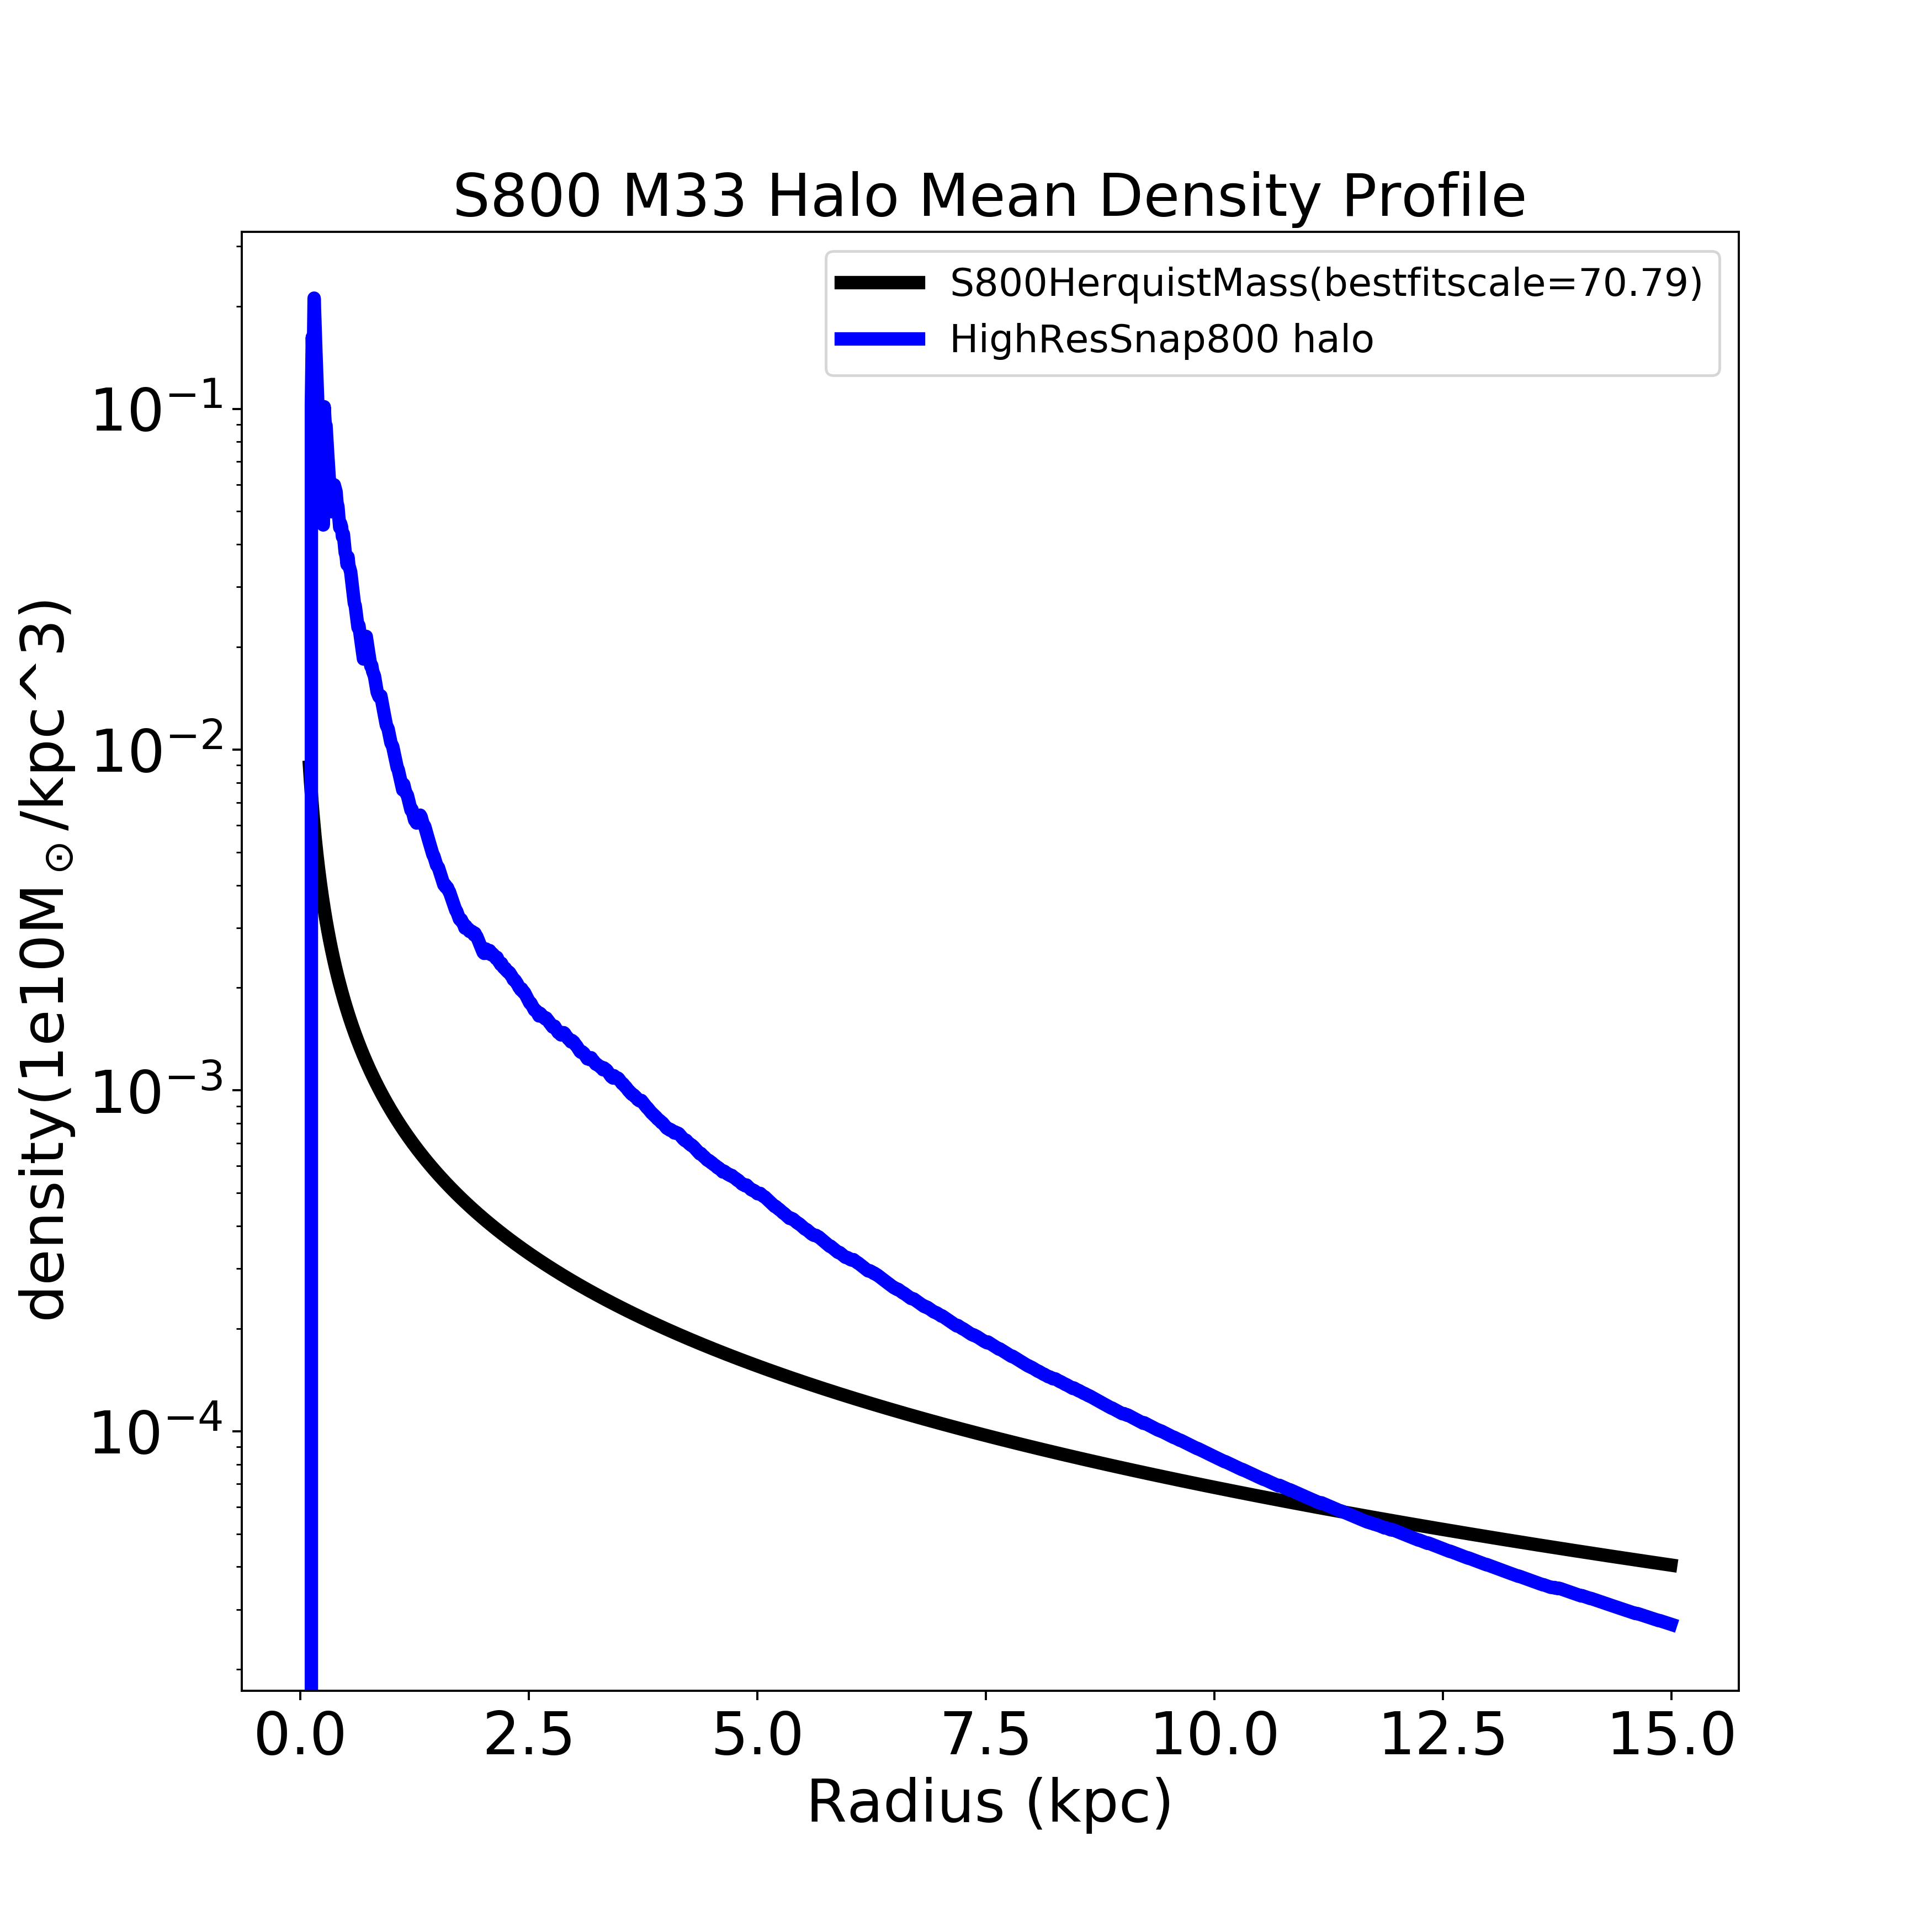
\includegraphics[width=2cm]{Snapshot800EnclosedVsHernquistMeanDensity.png}\hfill
    \\[\smallskipamount]
    \centering
    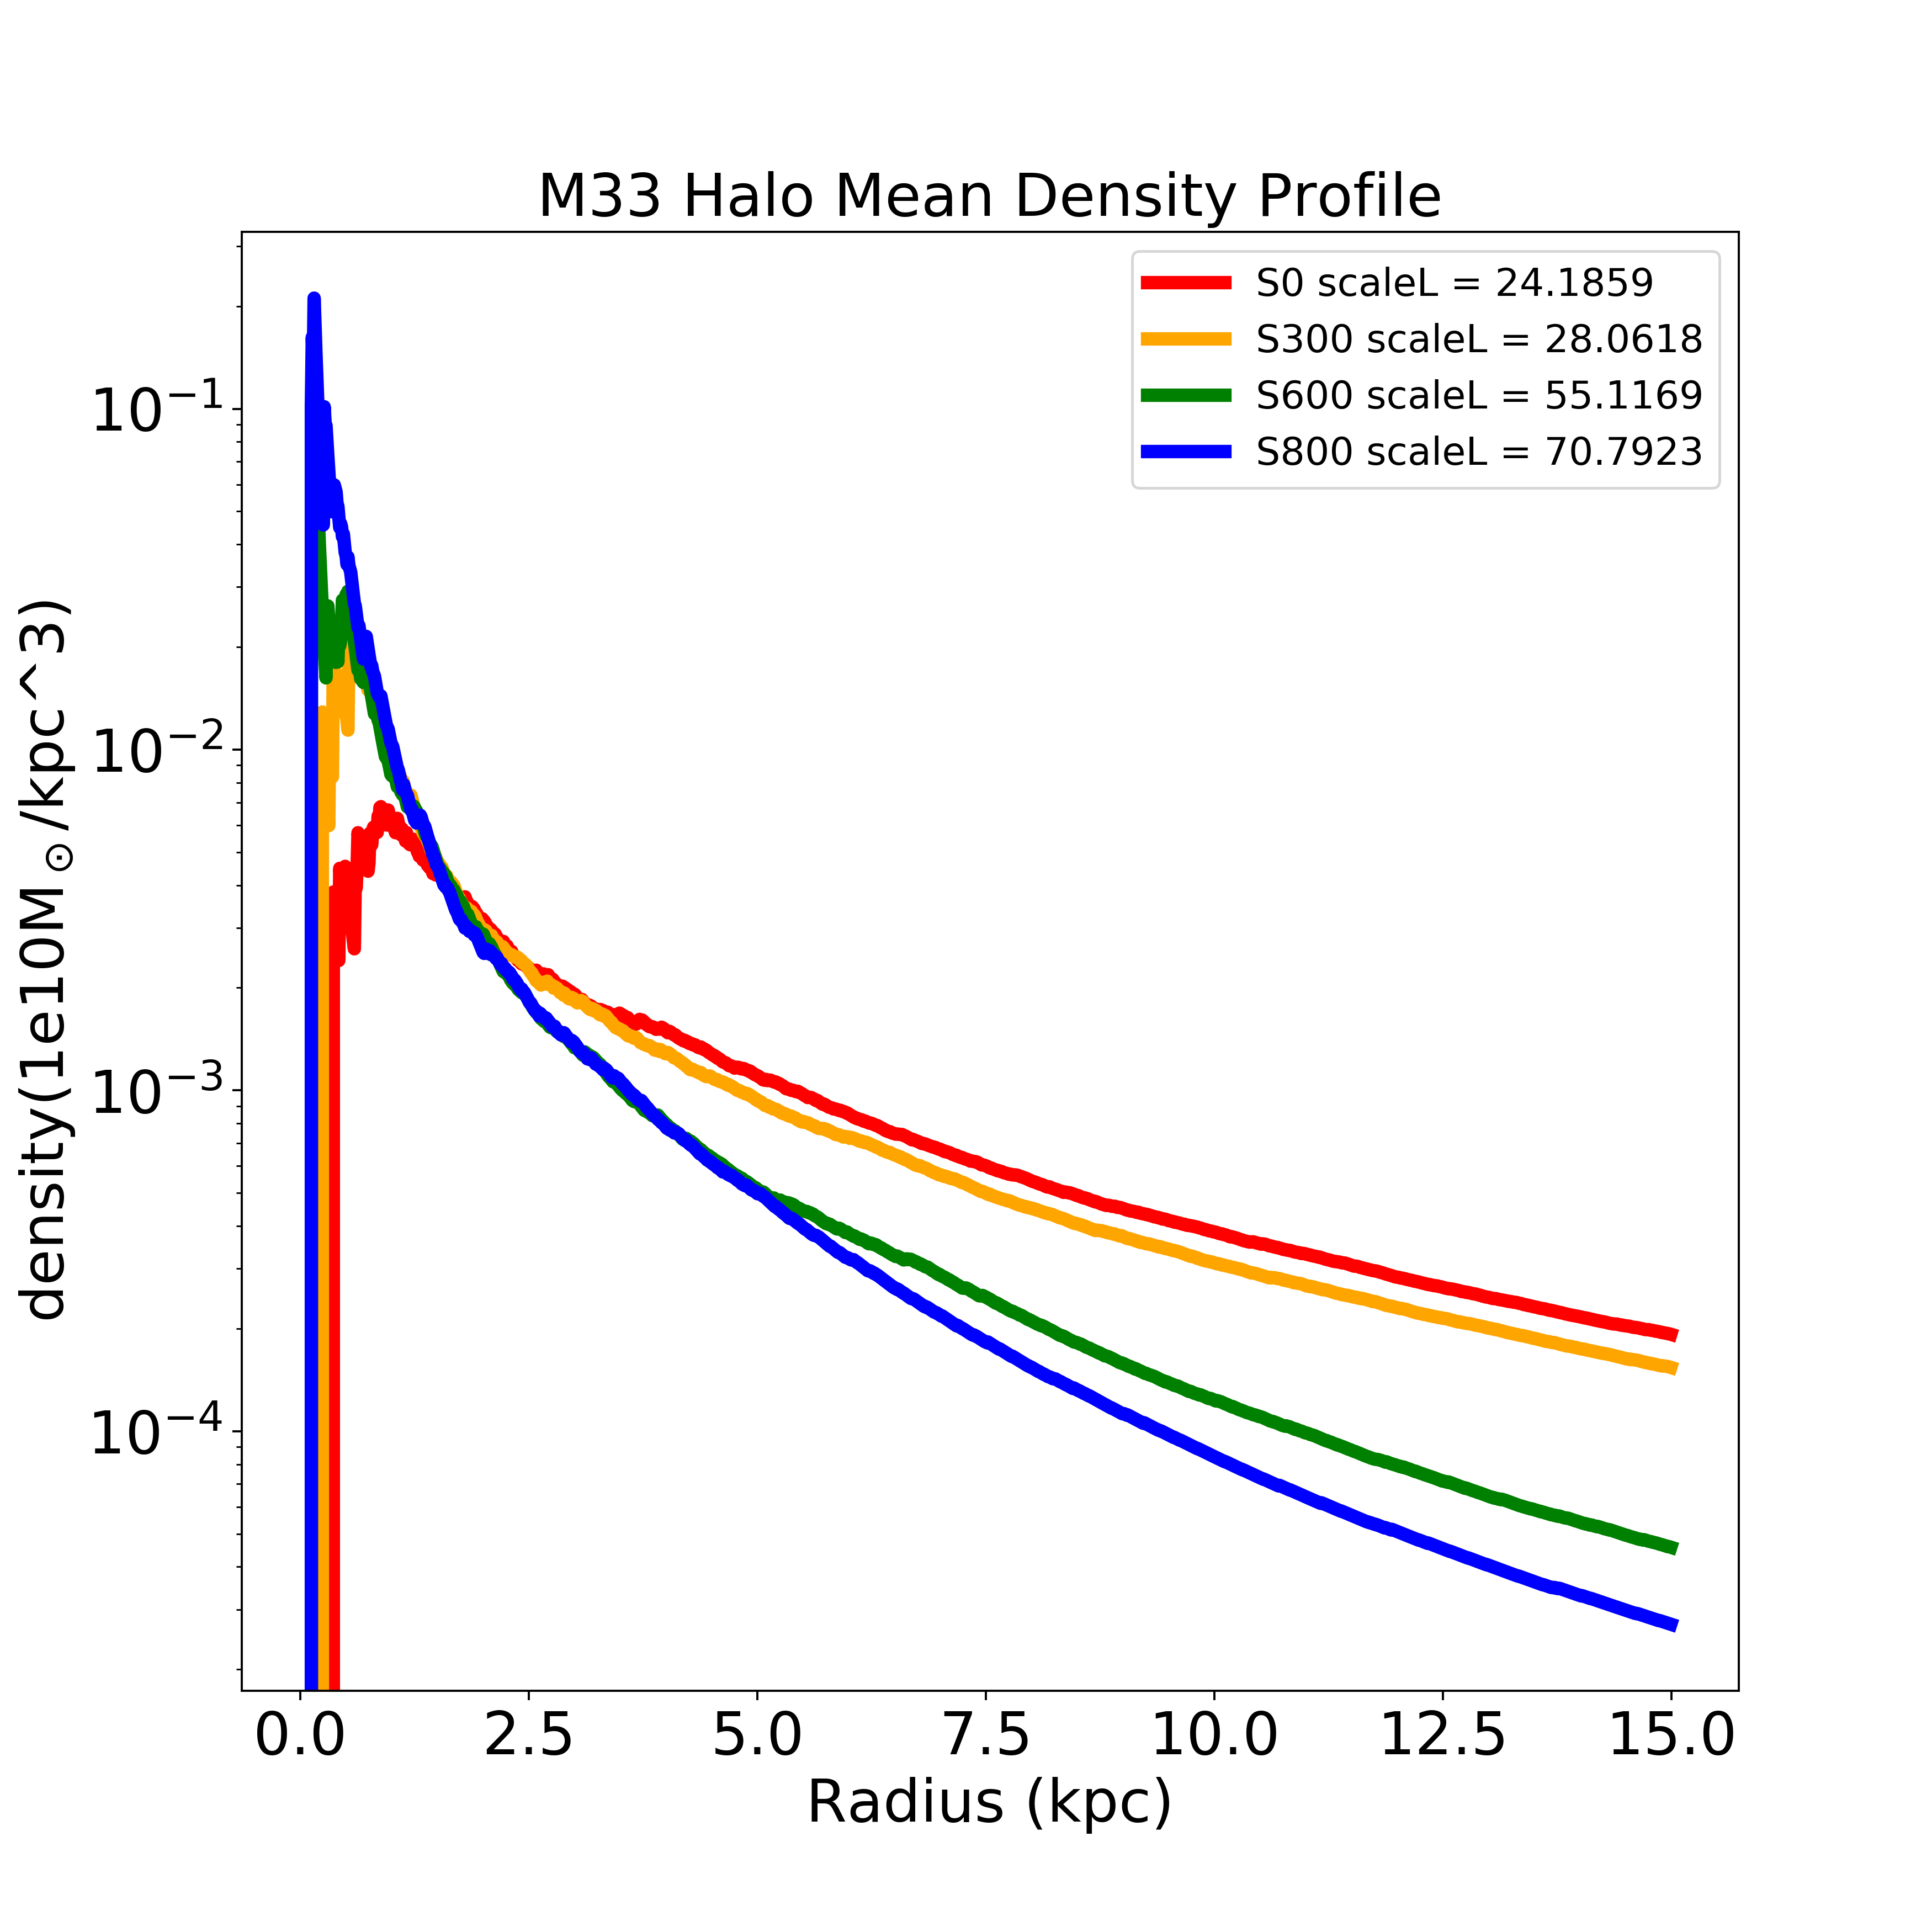
\includegraphics[width=3.5cm]{M33InternalMeanDensityProfile.png}
    \caption{The graph is the comparison of M33 internal dark matter mean density profiles and Hernquist mean density profile. The unit of y axis is 1e10solar mass per cubed kpc. And x axis is radius in kpc. 1.red represents snapshot0, 2.orange represents snapshot300, 3.green represents snapshot580, and 4.blue represents snapshot800. Black represents Hernquist mean density profile with best fitted scale length:1. 24.1859, 2. 28.0618, 3. 55.1169 and 4. 70.79.}
    \end{figure}
\section{Discussion}
\indent As indicated in the result of this paper, the part of M33 mass will lose in the future, due to the tidal effect which is from the Local Group (M31&MW&M33 system) acting on M33. The dark matter halo mass profile of M33 will change due to the orbit change of M31 and M33. As indicated in Figure 4, Jacobi radius of M31&M33 orbit aphelion is larger than it is when M33 is at its perihelion. Therefore, the mass loss rate is higher when M33 is close to M31 or the merger of M31 and MW; the mass loss rate is lower when M33 is far from M31 or the merger. In addition, the mass loss rate which is positive caused by the dark matter is passing through M33. The overall trend of M33 mass loss rate and dark matter halo profiles indicated that the gravitational well and depth of M33 will decrease in the future, especially after the merger of M31 and MW. It is not surprising to believe that M33 will accrete less gas and hold less baryons. M33 will lose in this "gravitational vs self balanced " battle to M31 and MW, because most of M33's dark matter will be striped.\\
\indent Furthermore, it is hard to detect dark matter annihilation in M33. As indicated in the M33 Hernquist mean density profiles on Figure 8, the dark matter mean density of M33 will keep decreasing in the future. As Boylan-Kolchin(2011) pointed that if the dark matter density of a galactic center is too low, astronomers could not observe any dark matter annihilation\citep{boylan11}. Therefore, there is no such a scientific value for searching on M33 in the future. 
\section{Conclusions}
This project shows the tidal evolution of M33&M31&MW system impact the M33 dark matter halo resulting in the mass loss of M33 dark Matter and change of M33 internal dark matter profile. The future evolution of M33 can be predicted as that M33 will keep shrinking in size and losing dark matters. Because the outcomes,which are from the Jacobi Radius simulation and Hernquist mean density profile, are tenable to support the conclusions of this project. The Jacobi Radius simulation reflects the change of M33 Jacobi Radius as function of time and the trend of M33 mass loss rate as function of average time. The simulation of Hernquist and Enclosed mass profile produced the graph of the M33 internal dark matter profile.     \\
\indent The change of the M33 dark matter mass profiles and mass loss rate demonstrate that M33 will keep losing dark matters in future. The change of Jacobi Radius and M33 mass profile can prove that the morphology and kinematics structures of M33 will consequently change. Therefore, the outcomes above agree with the hypothesis of this project that M33 will keep shrinking in size and losing dark matters.\\
\indent Additionally, the change of M33 internal dark mean density profile and Hernquist mean density profile indicate that M33's internal dark matter density will not be dense enough to produce dark matter annihilation in the future. So it will be hard for astronomers to search dark matter annihilation signals in order to do future dark matter experiments. \\
\indent The results of this project are based on the simulation data of M31M33MW orbit(provided by Gurtina Besla). As indicated in Figure 7, the actual Jacobi Radius of M33 is larger, and the dark matter mass loss rate of M33 is actually smaller due to the result of Hernquist Profile. As the further investigation of the topic, I can explore where the loss mass of M33 dark matters goes, the merger of M31 and MW or elsewhere? 
\section{Acknowledgements}
Thanks Prof.Besla and Rixin for helping. And those sources helped me to build my code:\\
\indent 1.Astropy,Astropy Collaboration et al. 2013; Price-Whelan et al. 2018 DOI:10.3847/15383881/aabc4f\\
\indent 2.matplotlib Hunter(2007),doi:10.1109/MCSE.2007.55\\
\indent 3.numpy van der Walt et al.(2011),DOI
:10.1109/MCSE.2011.37\\
\indent 4.scipy Jones et al(2001-),Open source scientific tools for Python. http://www.scipy.org/

\bibliography{final}{}
\bibliographystyle{aasjournal}

\end{document}
